% LuaLaTeX document — compile with: lualatex tmatrix_point_vs_galerkin.tex
% Then: biber tmatrix_point_vs_galerkin && lualatex tmatrix_point_vs_galerkin.tex
\documentclass[11pt,a4paper]{article}

\usepackage{fontspec}
\setmainfont{Latin Modern Roman}
\setmonofont{Latin Modern Mono}

\usepackage{amsmath,amssymb,amsthm,bm}
\usepackage{booktabs}
\usepackage{geometry}
\geometry{margin=2.5cm}
\usepackage[backend=biber,style=numeric,sorting=none]{biblatex}
\addbibresource{references.bib}
\usepackage{hyperref}
\hypersetup{colorlinks=true,linkcolor=blue!60!black,citecolor=green!50!black,urlcolor=blue!70!black}
\usepackage{enumitem}
\usepackage{xcolor}
\usepackage{mathtools}
\usepackage{graphicx}
\usepackage{tikz}
\usetikzlibrary{arrows.meta,calc,decorations.pathmorphing,shapes.geometric,positioning}
\usepackage{pgfplots}
\pgfplotsset{compat=1.18}
\pgfplotsset{table/search path={evidence/tables}}

% --- Macros (copied verbatim from docs/cube_galerkin27.tex) ---
\newcommand{\D}{\Delta}
\newcommand{\order}{\mathcal{O}}
\newcommand{\bG}{\bm{G}}
\newcommand{\bs}{\bm{s}}
\newcommand{\br}{\bm{r}}
\newcommand{\bxi}{\bm{\xi}}
\newcommand{\be}{\bm{\varepsilon}}
\newcommand{\bu}{\bm{u}}
\newcommand{\bphi}{\bm{\varphi}}
\newcommand{\R}{\mathbb{R}}
\newcommand{\PV}{\mathrm{p.v.}}
\newcommand{\indV}{\chi_V}
\newcommand{\Lspace}{L^1_{\mathrm{loc}}}

% --- Theorem environments ---
\theoremstyle{plain}
\newtheorem{theorem}{Theorem}
\newtheorem{proposition}[theorem]{Proposition}
\newtheorem{lemma}[theorem]{Lemma}
\theoremstyle{definition}
\newtheorem{definition}[theorem]{Definition}
\theoremstyle{remark}
\newtheorem{remark}[theorem]{Remark}

\title{Point-Source versus Body-Force Galerkin Representations of an
Elastic Cubic Scatterer:\\ a Mie- and Kennett-Validated Hierarchy}
\author{T.\,M.\ Nestor}
\date{June 2026}

\begin{document}
\maketitle

\begin{abstract}
\end{abstract}

\tableofcontents

\section{Introduction}\label{sec:intro}

\section{Background theory}\label{sec:background}

\subsection{Volume integral equation and the Lippmann--Schwinger formulation}
\label{sec:ls}

Consider an isotropic, homogeneous elastic background with Lam\'{e}
parameters $(\lambda_0,\mu_0)$, density $\rho_0$, and corresponding
Green's tensor $G_{ij}(\br)$ (the full elastodynamic propagator at
angular frequency $\omega$).  A finite inclusion $V\subset\mathbb{R}^3$
introduces contrasts $\D c_{nklj}$ in the stiffness tensor and $\D\rho$
in the density relative to the background.  The total displacement
$u_i(\br)$ satisfies the Lippmann--Schwinger (LS) volume integral
equation \cite{mura1987}:
\begin{equation}
  u_i(\br) \;=\; u_i^{0}(\br)
    + \omega^2\!\int_V G_{ij}(\br - \br')\,\D\rho\, u_j(\br')\,dV'
    - \int_V \partial'_k G_{in}(\br - \br')\,\D c_{nklj}\,
      \partial'_l u_j(\br')\,dV',
  \label{eq:LS}
\end{equation}
where $u_i^0$ is the incident displacement and the primed derivative
$\partial'_k$ acts on the source variable $\br'$.  The first integral
represents the body-force coupling through density contrast; the second
represents the elastic stiffness contrast through a double-gradient of
the Green's tensor.

The elastodynamic Green's tensor has the near-field singularity
structure
\begin{equation}
  G_{ij}(\bs) \sim |\bs|^{-1}, \qquad
  \partial G \sim |\bs|^{-2}, \qquad
  \partial\partial G \sim |\bs|^{-3},
  \label{eq:singularities}
\end{equation}
so the body-force kernel $G_{ij}$ is locally integrable, but taking
field-point derivatives of the stiffness-contrast term introduces
increasingly singular kernels.  Evaluating the stiffness integral at
the field point inside $V$ requires either a Cauchy principal-value
regularization or, for quadratic and higher trial functions, Eshelby-type
delta-function corrections \cite{eshelby1957}.  This singular structure
is the central technical constraint that shapes the hierarchy of
approximations discussed in Section~\ref{sec:t9}.

The far-field amplitude radiated by an inclusion is compactly encoded in
the single-site T-matrix $T_0$, which maps the incident wave onto the
scattered field:
\begin{equation}
  u_i^{\rm sc}(\br) \;\sim\; G_{ij}(\br - \br_0)\,T_{0,jk}\,u_k^{\rm inc}(\br_0)
  \qquad (|\br - \br_0| \to \infty).
\end{equation}
When multiple inclusions are present, the coupled system is governed by
the Foldy--Lax equations \cite{foldy1945,lax1951}, in which $T_0$ feeds
the inter-site propagator $G_0(\br_{ij})$ (Figure~\ref{fig:single-vs-inter}).

\subsection{Exact reference solutions}
\label{sec:oracles}

All representations examined in this paper are validated against two
exact reference solutions, treated as oracles.

\paragraph{Elastic Mie sphere.}
For a spherical inclusion of radius $a$ and contrast
$(\D\lambda, \D\mu, \D\rho)$, the scattered displacement admits an
exact partial-wave (Mie) expansion \cite{yingtruell1956}.  An incident
$P$-wave along $\hat{\bm{z}}$ is decomposed into Legendre orders $n$;
at each order the Helmholtz decomposition yields a $4\times4$ boundary
system (displacement and traction continuity for $P$- and $SV$-channels)
whose Cramer-rule solution gives the scattered-field amplitudes
$a_n$ ($P$-to-$P$) and $b_n$ ($P$-to-$S$).  At finite contrast the
series converges for all $ka$; no linearization is invoked.

Effective contrasts are extracted from the partial-wave coefficients
by Legendre projection: the monopole $a_0$ yields the bulk-modulus
contrast, the dipole $a_1$ yields the density contrast, and the
quadrupole $a_2$ yields the shear-modulus contrast.  These
Mie-reconstructed values serve as the ground-truth targets against
which point and Galerkin representations are compared in
Sections~\ref{sec:single}--\ref{sec:evidence}.

\paragraph{Kennett layered reflectivity.}
For the periodic-slab geometry, the exact specular P-to-P reflection
coefficient $R_{PP}$ is computed via the Kennett recursion \cite{kennett1983},
which assembles the full reflection matrix of a stratified medium using
propagator matrices and a generalized Bremmer series.  At normal
incidence with a single embedded layer of thickness $H$ and contrast
$(\D\lambda,\D\mu,\D\rho)$, the Kennett formula provides a
frequency-dependent $R_{PP}(\omega)$ valid at all contrasts.  This
serves as the slab oracle in Section~\ref{sec:evidence}.

Both references are free of any T-matrix approximation and are therefore
well-suited as error baselines: any discrepancy between a representation
and an oracle is a measure of that representation's truncation error.

\subsection{The single-site hierarchy}
\label{sec:hierarchy}

The paper compares three single-site representations of a cubic scatterer,
ordered below by increasing model complexity and computational cost
(Figure~\ref{fig:ladder}).  Whether this added complexity reduces the
observable far-field error is the central question, answered in
Section~\ref{sec:evidence}.

\begin{enumerate}[leftmargin=2em,label=\arabic*.]
  \item \textbf{Born / point-source.}  The simplest approximation
    replaces the internal field by the incident field,
    $u_j(\br') \approx u_j^0(\br')$, and integrates directly.  This
    gives a strength proportional to $V\D c$ or $V\omega^2\D\rho$,
    with no self-interaction.  The result is the leading-order Born
    scattering amplitude: a point source with volume-weighted contrast
    but no radiation-reaction damping.

  \item \textbf{Eshelby-corrected point scatterer.}  The Born strength
    is renormalized by the on-site radiation reaction $\operatorname{Im}\Gamma_0$,
    where $\Gamma_0$ is the imaginary part of the volume-averaged
    background Green's tensor evaluated at zero separation.  This
    correction, which follows from the elastodynamic optical theorem,
    accounts for the energy radiated by the scatterer and is essential
    for the point representation to satisfy energy conservation at
    finite frequency.  The real part of $\Gamma_0$ encodes the static
    Eshelby concentration tensor \cite{eshelby1957}, which dresses the
    incident strain inside the inclusion.

  \item \textbf{Body-force Galerkin $T_9$.}  The LS equation
    \eqref{eq:LS} is projected onto the nine-dimensional trial space
    spanned by the three uniform displacement modes and the six
    independent strain modes.  Because the trial functions are
    polynomials of degree $\le 1$, the bilinear forms involve only the
    body-force integral $\int\!\!\int G_{ij}\,dV\,dV'$ (kernel
    $|\bs|^{-1}$, absolutely convergent) and the stiffness integral
    with one derivative $\int\!\!\int \partial'_k G_{in}\,dV\,dV'$
    (kernel $|\bs|^{-2}$, conditionally convergent via integration by
    parts to the surface).  No Eshelby delta correction is required:
    the Galerkin projection absorbs the singularity into well-posed
    five-dimensional surface integrals.  This is the lowest-order
    closure that correctly captures both displacement and strain
    amplification inside the cube, giving an $\order(ka)^2$ accurate
    T-matrix across the Rayleigh regime.
\end{enumerate}

A natural further rung---the 27-component Galerkin extension with
quadratic trial functions---is excluded here: it yields no
Mie-consistent single-site far-field gain and contributes
$\le 0.07\,\%$ inter-voxel coupling (Section~\ref{sec:inter}).

\begin{figure}[h]
\centering
% fig_ladder.tex — Ladder of approximations (bottom=worst, top=excluded)
% No \usetikzlibrary — relies on arrows.meta,calc,positioning loaded by main doc
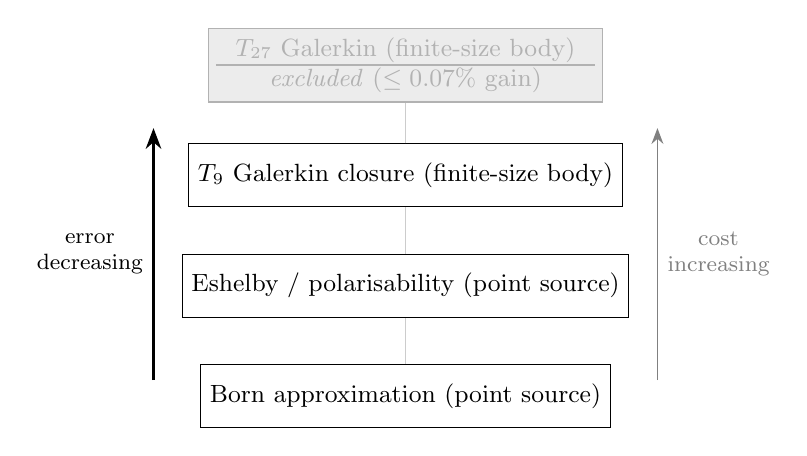
\begin{tikzpicture}[
  rung/.style={draw, fill=white, minimum width=5cm, minimum height=0.8cm,
               font=\small, align=center},
  excluded/.style={draw=gray!60, fill=gray!15, minimum width=5cm,
                   minimum height=0.8cm, font=\small\color{gray!70}, align=center,
                   text=gray!60},
  >=Stealth
]

% Rungs bottom to top
\node[rung] (born)    at (0,0)   {Born approximation (point source)};
\node[rung] (eshelby) at (0,1.4) {Eshelby / polarisability (point source)};
\node[rung] (t9)      at (0,2.8) {$T_9$ Galerkin closure (finite-size body)};
\node[excluded] (t27) at (0,4.2) {$T_{27}$ Galerkin (finite-size body) \\
                                   \textit{excluded} ($\le 0.07\%$ gain)};

% Strikethrough on excluded rung
\draw[gray!60, line width=0.8pt]
  ($(t27.west)+(0.1,0)$) -- ($(t27.east)+(-0.1,0)$);

% Vertical bracket / connecting lines between rungs
\foreach \bot/\top in {born/eshelby, eshelby/t9, t9/t27}{
  \draw[gray!40] (\bot.north) -- (\top.south);
}

% "Error decreasing" annotation on the left
\draw[->, line width=1pt]
  (-3.2,0.2) -- (-3.2,3.4)
  node[midway, left, font=\footnotesize, align=center] {error\\decreasing};

% "Complexity increasing" annotation on the right (optional, light)
\draw[->, line width=0.6pt, gray]
  (3.2,0.2) -- (3.2,3.4)
  node[midway, right, font=\footnotesize\color{gray}, align=center] {cost\\increasing};

\end{tikzpicture}

\caption{%
  Ladder of approximations from lowest (Born, point source) to the
  finite-size Galerkin closure $T_9$.  The $T_{27}$ rung is shown greyed and
  struck out because measurements show it contributes $\le 0.07\,\%$ gain over
  $T_9$ at all validated frequencies, making the added cost unjustified.
  Rungs are ordered by increasing model complexity and computational cost
  (Born $<$ Eshelby-point $<$ $T_9$).  Whether far-field accuracy follows
  this ordering is the question settled empirically in
  Section~\ref{sec:evidence}; it does not, for the single-site far field.%
}
\label{fig:ladder}
\end{figure}

\begin{figure}[h]
\centering
% fig_single_vs_inter.tex — Self-energy (single-site) vs inter-site coupling
% Libraries used: arrows.meta, calc, decorations.pathmorphing (for wavy loop)
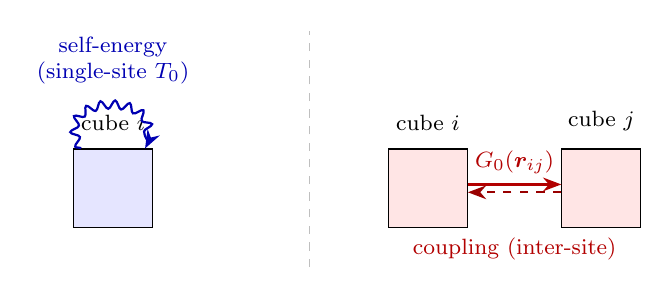
\begin{tikzpicture}[>=Stealth, font=\small]

% ---- Left panel: single cube with self-loop ----
\node[draw, fill=blue!10, minimum size=1.0cm] (cube1) at (-3,0) {};
\node[above=0.1cm of cube1, font=\footnotesize] {cube $i$};

% Self-loop arrow above the cube
\draw[->, thick, blue!70!black,
      decoration={snake, amplitude=1.5pt, segment length=5pt},
      decorate]
  ($(cube1.north west)+(0.1,0)$)
  .. controls (-3.8,1.2) and (-2.2,1.2) ..
  ($(cube1.north east)+(-0.1,0)$);
\node[above, yshift=1.2cm, font=\footnotesize, blue!70!black, align=center]
  at (cube1) {self-energy\\(single-site $T_0$)};

% ---- Right panel: two cubes with inter-site arrow ----
\node[draw, fill=red!10, minimum size=1.0cm] (cubeA) at (1.0,0) {};
\node[draw, fill=red!10, minimum size=1.0cm] (cubeB) at (3.2,0) {};
\node[above=0.1cm of cubeA, font=\footnotesize] {cube $i$};
\node[above=0.1cm of cubeB, font=\footnotesize] {cube $j$};

% Inter-site coupling arrow
\draw[->, thick, red!70!black]
  ($(cubeA.east)+(0,0.05)$) -- ($(cubeB.west)+(0,0.05)$)
  node[midway, above, font=\footnotesize, red!70!black] {$G_0(\br_{ij})$};
\draw[->, thick, red!60!black, dashed]
  ($(cubeB.west)+(0,-0.05)$) -- ($(cubeA.east)+(0,-0.05)$);

\node[below=0.5cm, font=\footnotesize, red!70!black, align=center]
  at ($(cubeA)!0.5!(cubeB)$) {coupling (inter-site)};

% Vertical divider
\draw[gray!50, dashed] (-0.5,-1.0) -- (-0.5,2.0);

\end{tikzpicture}

\caption{%
  Single-site self-energy (left: scatterer $i$ radiates back into itself,
  captured by $T_0$) versus inter-site coupling (right: wave field propagates
  from scatterer $i$ to $j$ via the background Green tensor $G_0(\br_{ij})$
  and back).  The Foldy-Lax system couples both contributions.%
}
\label{fig:single-vs-inter}
\end{figure}

\section{The body-force Galerkin closure (\texorpdfstring{$T_9$}{T9})}\label{sec:t9}

\subsection{Galerkin projection onto the polynomial trial space}
\label{sec:t9-galerkin}

Let $V = [-a,a]^{3}$ be the cubic inclusion.  The \emph{nine-dimensional
trial space}
\begin{equation}
  T_9 \;=\; \bigl\{\,\bphi(\br) \;\big|\;
  \varphi_i(\br) = U_i + \varepsilon_{ai}\,r_a,\quad
  \varepsilon_{ai} = \varepsilon_{ia}\,\bigr\}
  \label{eq:T9-def}
\end{equation}
spans the three uniform-displacement modes ($3$ degrees of freedom from
$U_i$) and the six independent components of the symmetric strain tensor
($6$ degrees of freedom from $\varepsilon_{ai}$), giving $3+6=9$ trial
functions in total.  The trial functions are polynomials of total degree
$\le 1$ in $\br$.

\begin{definition}[$T_9$ Galerkin closure]
The $T_9$ closure is the variational problem: find $\bu^h \in T_9$ such
that for all $\bphi \in T_9$,
\begin{equation}
  \langle\bphi,\bu^h\rangle_V
  \;=\;
  \langle\bphi,\bu^{0}\rangle_V
  + \omega^{2}\D\rho\,\mathcal{B}_{\mathrm{body}}[\bphi,\bu^{h}]
  - \D c_{nklj}\,\mathcal{B}_{\mathrm{el}}[\bphi,\bu^{h}],
  \label{eq:galerkin-LS-T9}
\end{equation}
where the bilinear forms are
\begin{align}
\langle\bphi,\bu\rangle_V &:= \int_{V} \varphi_i(\br)\, u_i(\br)\,dV,
  \label{eq:mass-form} \\[3pt]
\mathcal{B}_{\mathrm{body}}[\bphi,\bu] &:= \int_{V}\!\!\int_{V}
  \varphi_i(\br)\,G_{in}(\br-\br')\,u_n(\br')\,dV\,dV',
  \label{eq:body-form} \\[3pt]
\mathcal{B}_{\mathrm{el}}[\bphi,\bu] &:= \int_{V}\!\!\int_{V}
  \varphi_i(\br)\,\partial'_k G_{in}(\br-\br')\,
  \partial'_l u_j(\br')\,dV\,dV'.
  \label{eq:elastic-form}
\end{align}
\end{definition}

\paragraph{Why $T_9$ is singularity-free.}
This is the central structural advantage of the Galerkin formulation at
degree~$\le 1$.  The body-force form $\mathcal{B}_{\mathrm{body}}$
involves only the Green's tensor itself, with kernel $|\bs|^{-1}$, which
is locally integrable in $\R^{6}$ by the Hardy--Littlewood--Sobolev
inequality.  For the elastic form $\mathcal{B}_{\mathrm{el}}$, since
$\bu \in T_9$ is a degree-$\le 1$ polynomial, we may integrate by parts
on the trial function $\bu$:
\begin{equation}
  \mathcal{B}_{\mathrm{el}}[\bphi,\bu]
  \;=\;
  -\int_{V}\!\!\int_V\!\varphi_i\,G_{in}\,
    \underbrace{\partial'_k\partial'_l u_j}_{=0}\,dV'\,dV
  + \int_{V}\!\!\oint_{\partial V}\!\varphi_i\,G_{in}\,
    \partial'_l u_j\,n_k\,dS'\,dV.
  \label{eq:ibp-elastic}
\end{equation}
Because degree-$\le 1$ functions have zero second derivative, the volume
term vanishes exactly and $\mathcal{B}_{\mathrm{el}}$ reduces to a
five-dimensional surface integral against the $|\bs|^{-1}$ kernel (not
$|\bs|^{-2}$ or worse).  Both bilinear forms therefore involve only
absolutely convergent integrals.

\begin{proposition}[Well-posedness]\label{prop:wellposed-T9}
For $\bphi, \bu \in T_9$, every bilinear form in
\eqref{eq:galerkin-LS-T9} is finite.  No Cauchy principal-value
regularization, no Eshelby-type delta-function correction, and no
distributional bookkeeping is required.
\end{proposition}

Table~\ref{tab:singularities-T9} summarizes the contrast with the
point-evaluation (Path~A) closure, where taking field-point derivatives
of the Green's tensor inside $V$ introduces increasingly singular
kernels.

\begin{table}[h]
\centering
\begin{tabular}{lll}
\toprule
Contribution & Worst kernel & $T_9$ Galerkin status \\
\midrule
Body-force $\mathcal{B}_{\mathrm{body}}$ & $1/|\bs|$ & $\Lspace$ --- absolutely convergent \\
Elastic $\mathcal{B}_{\mathrm{el}}$ (after IBP) & $1/|\bs|$ & surface integral, absolutely convergent \\
Path-A strain evaluation & $1/|\bs|^{2}$ & principal-value regularization needed \\
Path-A gradient evaluation & $1/|\bs|^{3}$ & Eshelby delta correction needed \\
\bottomrule
\end{tabular}
\caption{Singular structure for the $T_9$ Galerkin closure vs.\ the
point-evaluation (Path~A) closure.  The Galerkin projection absorbs the
singularity into a well-posed surface integral, removing the need for
distributional corrections.}
\label{tab:singularities-T9}
\end{table}

\subsection{Centre-of-mass and relative-coordinate reduction}
\label{sec:t9-cm}

The six-fold double integral in $\mathcal{B}_{\mathrm{body}}$ is reduced to
a three-fold integral by the change of variables
\begin{equation}
  \bxi = \tfrac{1}{2}(\br + \br'), \qquad \bs = \br - \br',
  \qquad d\br\,d\br' = d\bxi\,d\bs,
  \label{eq:cm-vars}
\end{equation}
known in the Eshelby--Mura literature as sum-and-difference variables
\cite{eshelby1957,mura1987}.  The constraint $\br,\br' \in V$ restricts
$\bxi$ to a centred box of half-widths $a - |s_i|/2$ in each direction.
Integrating out $\bxi$ yields
\begin{equation}
  \int_{V}\!\!\int_{V}\!\varphi_i(\br)\,K(\br-\br')\,u_n(\br')\,d\br\,d\br'
  \;=\; \int_{[-2a,2a]^{3}}\!K(\bs)\,
    \Big[\int_{B(\bs)}\!\varphi_i\!\bigl(\bxi+\tfrac{\bs}{2}\bigr)\,
         u_n\!\bigl(\bxi-\tfrac{\bs}{2}\bigr)\,d\bxi\Big]\,d\bs,
  \label{eq:cm-reduction}
\end{equation}
where the inner bracket is a polynomial in $(\bs, a)$ for polynomial
$\bphi, \bu$.  For the case $\bphi = \bu = \mathbf{1}$ (constant modes),
the inner integral is exactly the \emph{cube autocorrelation}
\begin{equation}
  \Lambda_V(\bs) \;=\; (\indV \star \indV)(\bs)
  \;=\; \prod_{i=1}^{3}(2a - |s_i|)_+,
  \label{eq:tent}
\end{equation}
the three-dimensional tent function with support $|s_i| \le 2a$
(Figure~\ref{fig:cm-relative}).  For the linear (strain) modes the inner
integral contributes additional polynomial factors that multiply the tent.
The final outer integral has the form
\begin{equation}
  \text{polynomial}(\bs)\times |\bs|^{-1}
  \quad \text{or} \quad
  \text{polynomial}(\bs)\times s_i s_j\,|\bs|^{-3},
\end{equation}
over $[-2a,2a]^3$, which by rescaling $\bs = 2a\,\bu$ becomes the
master integrals of Appendix~\ref{app:masters}.

\begin{figure}[h]
\centering
% fig_cm_relative.tex — Two overlapping cubes: CM vector xi, relative vector s
%                        plus inset tent function Lambda_V(s)
% Libraries: arrows.meta, calc
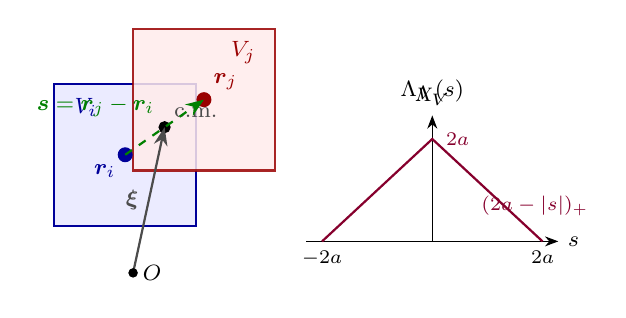
\begin{tikzpicture}[>=Stealth, font=\small]

% ---- Two overlapping cubes ----
% Cube 1 (bottom-left, blue)
\draw[blue!60!black, thick, fill=blue!8]
  (-1.0, -0.6) rectangle (0.8, 1.2);
\node[blue!60!black, font=\footnotesize] at (-0.6, 0.9) {$V_i$};

% Cube 2 (top-right, red), partially overlapping
\draw[red!60!black, thick, fill=red!8, opacity=0.85]
  (-0.0, 0.1) rectangle (1.8, 1.9);
\node[red!60!black, font=\footnotesize] at (1.4, 1.6) {$V_j$};

% Centres
\coordinate (ci) at (-0.1, 0.3);   % centre of cube i
\coordinate (cj) at (0.9,  1.0);   % centre of cube j

\filldraw[blue!60!black] (ci) circle (2.5pt) node[below left, font=\footnotesize] {$\br_i$};
\filldraw[red!60!black]  (cj) circle (2.5pt) node[above right, font=\footnotesize] {$\br_j$};

% CM vector xi = (r_i + r_j)/2
\coordinate (cm) at ($(ci)!0.5!(cj)$);
\filldraw[black] (cm) circle (2pt);
\draw[->, thick, black!70]
  (0, -1.2) -- (cm)
  node[midway, left, font=\footnotesize] {$\bxi$};
\node[above right, font=\footnotesize, black!70] at (cm) {c.m.};

% Relative vector s = r_j - r_i
\draw[->, thick, green!50!black, dashed]
  (ci) -- (cj)
  node[midway, above left, font=\footnotesize, green!50!black] {$\bs = \br_j - \br_i$};

% Origin
\filldraw[black] (0,-1.2) circle (1.5pt) node[right, font=\footnotesize] {$O$};

% ---- Inset: tent function Lambda_V(s) ----
\begin{scope}[xshift=3.8cm, yshift=-0.8cm]
  \draw[->] (-1.6,0) -- (1.6,0) node[right, font=\footnotesize] {$s$};
  \draw[->] (0,0)    -- (0,1.6) node[above, font=\footnotesize] {$\Lambda_V$};
  % Tent function: peak at 0, zero at ±2a
  \draw[thick, purple!70!black]
    (-1.4, 0) -- (0, 1.3) -- (1.4, 0);
  % Labels
  \node[below, font=\scriptsize] at (-1.4, 0) {$-2a$};
  \node[below, font=\scriptsize] at ( 1.4, 0) {$2a$};
  \node[right, font=\scriptsize, purple!70!black] at (0.05, 1.3) {$2a$};
  \node[below right, font=\scriptsize, purple!70!black] at (0.5, 0.7)
    {$(2a - |s|)_+$};
  \node[above, font=\footnotesize, align=center] at (0, 1.65)
    {$\Lambda_V(s)$};
\end{scope}

\end{tikzpicture}

\caption{%
  Centre-of-mass coordinate $\bxi = \tfrac{1}{2}(\br_i + \br_j)$ and
  relative coordinate $\bs = \br_j - \br_i$ for a pair of overlapping unit
  cells $V_i$, $V_j$.  Inset: the tent (triangular) overlap kernel
  $\Lambda_V(s) = (2a - |s|)_+$ that emerges from the volume convolution,
  with support $|s| \le 2a$.%
}
\label{fig:cm-relative}
\end{figure}

\subsection{Closed-form effective contrasts from the $T_9$ closure}
\label{sec:t9-contrasts}

Solving the $9\times9$ linear system \eqref{eq:galerkin-LS-T9} yields
the internal displacement amplitude $\bu^h$ inside the cube.  Under cubic
($O_h$) symmetry the system block-diagonalises into two independent sectors:

\paragraph{Displacement sector (3 modes, ungerade).}
The three uniform-displacement modes decouple from the strain modes by
parity.  Their T-matrix amplitude is driven by the density contrast
$\omega^2\D\rho$ via the body bilinear form and gives the effective
density contrast
\begin{equation}
  \D\rho^{*}
  \;=\; A_u\,\D\rho, \qquad
  A_u \;=\; \frac{1}{1 - \omega^2\D\rho\,\Gamma_0},
  \label{eq:Arho}
\end{equation}
where $\Gamma_0$ is the real part of the volume-averaged body bilinear
evaluated on the displacement sector:
\begin{equation}
  \Gamma_0 \;=\; \frac{1}{V}\,\mathcal{B}_{\mathrm{body}}[\mathbf{e}_i, \mathbf{e}_i]
  \quad\text{(no sum on }i\text{)}.
  \label{eq:Gamma0}
\end{equation}
The denominator factor $A_u$ is the self-consistent displacement
amplification inside the cube; it encodes the Eshelby concentration
effect \cite{eshelby1957} for the inertial (density) channel.  In the
static limit $\omega\to 0$ (or $\D\rho\to 0$), $A_u\to 1$ and
$\D\rho^{*} \to \D\rho$.

\paragraph{Strain sector (6 modes, gerade).}
The six symmetric-strain modes carry the stiffness contrast
$(\D\lambda, \D\mu)$.  The elastic bilinear form
$\mathcal{B}_{\mathrm{el}}$ (eq.~\eqref{eq:elastic-form}) on
$T_9$ is block-diagonal with the mass form by parity: the
displacement--strain cross block is identically zero (odd integrand on the
symmetric cube).  The strain-sector Galerkin eigenproblem yields the
self-consistent effective Lam\'e contrasts
\begin{align}
  \D\lambda^* &= \bigl(\D\lambda + \tfrac{2}{3}\D\mu\bigr)\,A_\theta
    - \tfrac{2}{3}\D\mu\,A_e,
    \label{eq:Dlambda-star-T9}\\
  \D\mu^* &= \D\mu\cdot A_e,
  \label{eq:Dmu-star-T9}
\end{align}
where $A_\theta$ and $A_e$ are the volumetric and deviatoric amplification
factors from the Eshelby concentration tensor \cite{eshelby1957,mura1987}.
The cross-term in \eqref{eq:Dlambda-star-T9} couples the bulk and
deviatoric channels.  Unlike the displacement sector, the strain sector
has no dynamic ($\omega^2$) prefactor at leading Rayleigh order: the
stiffness channel is governed by the static Eshelby geometry.

\paragraph{Remark on cubic anisotropy.}
The $T_9$ elastic bilinear restricted to the strain sector has
irreducible eigenvalues $8(3\D\lambda+2\D\mu)$, $16\D\mu$, and $8\D\mu$
on the $A_{1g}$, $E_g$, and $T_{2g}$ irreps respectively.  The equality
of the $E_g$ and $T_{2g}$ eigenvalues in the stiffness channel means the
$T_9$ strain block is strictly isotropic---cubic anisotropy of the cube
T-matrix arises through the $B$-channel of the body bilinear
(the $s_i s_j/|\bs|^3$ kernel acting on the displacement sector coupled
back to the strain) and is a subleading effect in the Rayleigh regime.

The numerical values of $\Gamma_0$, $A_\theta$, and $A_e$ follow from
the master integrals in Appendix~\ref{app:masters}; the complete closed
forms are given there.

\section{Single-site self-energy corrections}\label{sec:single}

\begin{figure}[h]
\centering
% fig_ldos.tex — Radiation patterns: point force vs moment tensor (LDOS)
% Libraries: arrows.meta, calc
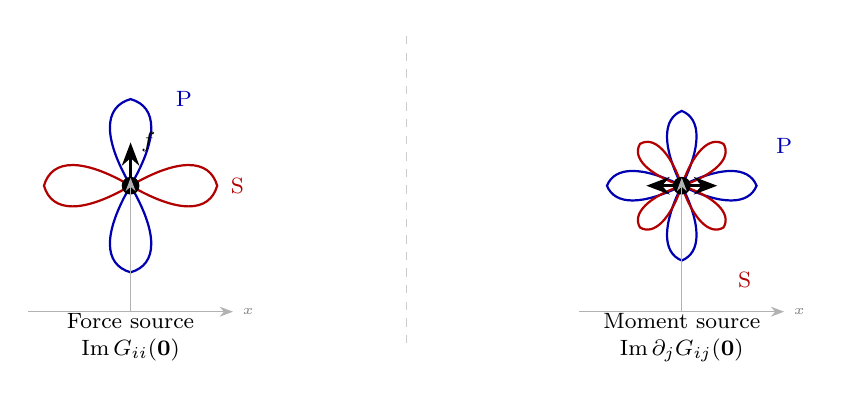
\begin{tikzpicture}[>=Stealth, font=\small]

% =========================================================
% LEFT: point FORCE — radiates into 1P + 2S lobes
% P-wave lobe: cos²θ (figure-eight along z)
% S-wave lobe: sin²θ (torus cross-section)
% We draw schematic outlines only
% =========================================================

\begin{scope}[xshift=-3.5cm]
  % P-wave lobes (figure-eight, vertical)
  \draw[blue!70!black, thick]
    (0,0) .. controls ( 0.35, 0.6) and ( 0.35, 1.0) .. (0, 1.1)
          .. controls (-0.35, 1.0) and (-0.35, 0.6) .. (0, 0);
  \draw[blue!70!black, thick]
    (0,0) .. controls ( 0.35,-0.6) and ( 0.35,-1.0) .. (0,-1.1)
          .. controls (-0.35,-1.0) and (-0.35,-0.6) .. (0, 0);
  \node[blue!70!black, font=\footnotesize, right] at (0.45, 1.1) {P};

  % S-wave lobes (figure-eight, horizontal)
  \draw[red!70!black, thick]
    (0,0) .. controls (0.6,  0.35) and (1.0,  0.35) .. (1.1, 0)
          .. controls (1.0, -0.35) and (0.6, -0.35) .. (0,   0);
  \draw[red!70!black, thick]
    (0,0) .. controls (-0.6,  0.35) and (-1.0,  0.35) .. (-1.1, 0)
          .. controls (-1.0, -0.35) and (-0.6, -0.35) .. ( 0,   0);
  \node[red!70!black, font=\footnotesize, right] at (1.15, 0) {S};

  % Force source
  \filldraw[black] (0,0) circle (3pt);
  \draw[->, very thick] (0,0) -- (0, 0.55) node[right, font=\footnotesize] {$f$};

  \node[below=1.5cm, align=center, font=\footnotesize]
    at (0,0) {Force source\\$\mathrm{Im}\, G_{ii}(\mathbf{0})$};
\end{scope}

% =========================================================
% RIGHT: DIPOLE / moment tensor — P monopole+quadrupole, S quadrupole
% Schematic: "donut" S lobes at 45°, P lobes along axes
% =========================================================

\begin{scope}[xshift=3.5cm]
  % P lobes along ±z and ±x (quadrupole shape — 4 lobes)
  \foreach \ang in {0, 90, 180, 270}{
    \begin{scope}[rotate=\ang]
      \draw[blue!70!black, thick]
        (0,0) .. controls (0.25, 0.5) and (0.25, 0.85) .. (0, 0.95)
              .. controls (-0.25, 0.85) and (-0.25, 0.5) .. (0, 0);
    \end{scope}
  }
  \node[blue!70!black, font=\footnotesize] at (1.3, 0.5) {P};

  % S lobes at 45° (quadrupole)
  \foreach \ang in {45, 135, 225, 315}{
    \begin{scope}[rotate=\ang]
      \draw[red!70!black, thick]
        (0,0) .. controls (0.2, 0.4) and (0.2, 0.7) .. (0, 0.75)
              .. controls (-0.2, 0.7) and (-0.2, 0.4) .. (0, 0);
    \end{scope}
  }
  \node[red!70!black, font=\footnotesize] at (0.8, -1.2) {S};

  % Moment tensor source
  \filldraw[black] (0,0) circle (3pt);
  % Small double-headed arrow to indicate dipole/moment
  \draw[<->, very thick] (-0.45,0) -- (0.45,0);

  \node[below=1.5cm, align=center, font=\footnotesize]
    at (0,0) {Moment source\\$\mathrm{Im}\, \partial_j G_{ij}(\mathbf{0})$};
\end{scope}

% Panel divider
\draw[gray!40, dashed] (0,-2.0) -- (0, 2.0);

% Overall x-axis reference
\foreach \panel in {-3.5, 3.5}{
  \draw[gray!60, ->] (\panel-1.3, -1.6) -- (\panel+1.3, -1.6)
    node[right, font=\tiny, gray] {$x$};
  \draw[gray!60, ->] (\panel, -1.6) -- (\panel, 0.1);
}

\end{tikzpicture}

\caption{%
  Schematic radiation patterns entering the local density of states (LDOS).
  Left: a point \emph{force} source radiates into a dipolar P lobe
  ($\cos^2\!\theta$) and two transverse S lobes ($\sin^2\!\theta$),
  proportional to $\operatorname{Im} G_{ii}(\mathbf{0})$.
  Right: a \emph{moment-tensor} (dipole) source produces quadrupolar P and S
  patterns, proportional to $\operatorname{Im} \partial_j G_{ij}(\mathbf{0})$.
  The imaginary parts of these on-site Green tensor components determine
  the radiation-reaction correction to the effective single-site T-matrix.%
}
\label{fig:ldos}
\end{figure}

\section{Inter-site coupling}\label{sec:inter}

\begin{figure}[h]
\centering
% fig_intersite_phase.tex — Two stacked cells, vertical coupling arrow +
%                            horizontal phase ramp / wavy arrow
% Libraries: arrows.meta, calc, decorations.pathmorphing
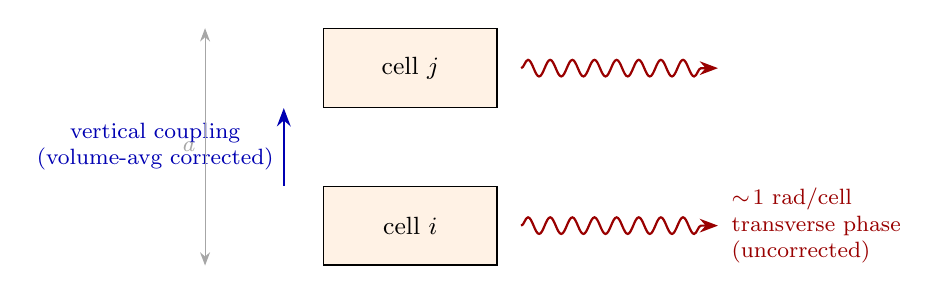
\begin{tikzpicture}[>=Stealth, font=\small]

% ---- Two stacked cells (vertical) ----
\node[draw, fill=orange!10, minimum width=2.2cm, minimum height=1.0cm,
      label=center:cell $j$] (cellB) at (0, 0)   {};
\node[draw, fill=orange!10, minimum width=2.2cm, minimum height=1.0cm,
      label=center:cell $i$] (cellA) at (0, -2.0) {};

% ---- Vertical coupling arrow (left side) ----
\draw[->, thick, blue!70!black]
  ($(cellA.north west)+(-0.5, 0)$) -- ($(cellB.south west)+(-0.5, 0)$)
  node[midway, left, font=\footnotesize, blue!70!black, align=center]
  {vertical coupling\\(volume-avg corrected)};

% ---- Wavy horizontal arrow (right side) — transverse phase ----
\draw[->, thick, red!60!black,
      decoration={snake, amplitude=3pt, segment length=8pt, post length=4pt},
      decorate]
  ($(cellA.east)+(0.3, 0)$) -- ($(cellA.east)+(2.8, 0)$);
\node[right, font=\footnotesize, red!60!black, align=left]
  at ($(cellA.east)+(2.85, 0)$) {$\sim\!1$ rad/cell\\transverse phase\\(uncorrected)};

% Also show the wavy arrow for the upper cell at same horizontal offset
\draw[->, thick, red!60!black,
      decoration={snake, amplitude=3pt, segment length=8pt, post length=4pt},
      decorate]
  ($(cellB.east)+(0.3, 0)$) -- ($(cellB.east)+(2.8, 0)$);

% ---- Lattice pitch label ----
\draw[<->, gray!70]
  ($(cellA.south west)+(-1.5, 0)$) -- ($(cellB.north west)+(-1.5, 0)$)
  node[midway, left, font=\footnotesize, gray!70] {$a$};

\end{tikzpicture}

\caption{%
  Two vertically adjacent unit cells illustrating the two dominant
  inter-site coupling effects.  The vertical (out-of-plane) coupling arrow
  (blue, left) is corrected by the volume-average of the Green tensor over
  the cell pair, removing the $1/r$ singularity.  The horizontal wavy arrow
  (red, right) represents $\sim\!1$ rad/cell transverse phase accumulation
  that is \emph{not} corrected by the volume average and drives the
  convergence criterion $ka \ll 1$ for the quasi-static Galerkin scheme.%
}
\label{fig:intersite-phase}
\end{figure}

\section{Evidence synthesis and cost--accuracy}\label{sec:evidence}

\begin{figure}[htbp]
\centering
\begin{tikzpicture}
\begin{axis}[
  xlabel={$ka_S$}, ylabel={relative $L^2$ error vs.\ Mie},
  ymode=log, legend pos=north west, width=0.8\linewidth,
  grid=both, mark size=2pt]
  \addplot table[x=ka,y=l2]{error_vs_ka_born.dat};    \addlegendentry{Born (point)}
  \addplot table[x=ka,y=l2]{error_vs_ka_eshelby.dat};  \addlegendentry{Eshelby (point)}
  \addplot table[x=ka,y=l2]{error_vs_ka_t9.dat};       \addlegendentry{$T_9$ Galerkin}
\end{axis}
\end{tikzpicture}

\caption{Relative $L^2$ error vs.\ exact Mie for three point/Galerkin representations
  at moderate contrast, P-incidence, across the validated $ka_S$ sweep.
  Eshelby-corrected point scatterer is most accurate at all $ka$; bare Born
  carries the largest error; $T_9$ Galerkin lies between them.}
\label{fig:error-vs-ka}
\end{figure}

\section{Discussion and conclusion}\label{sec:conclusion}

\appendix
\section{Master integrals (\texorpdfstring{$T_9$}{T9} subset)}\label{app:masters}

After the centre-of-mass/relative reduction of Section~\ref{sec:t9-cm},
every entry of the $9\times 9$ Galerkin matrix is a finite linear
combination of two families of three-dimensional master integrals over the
unit cube $[0,1]^3$ (using octant symmetry $\bs \to \bu$, $|\bs|=2a|\bu|$):
\begin{align}
  \mathcal{M}^+_{p,q,r}
  &:= \int_{[0,1]^3}\!\frac{x^p\,y^q\,z^r}{\sqrt{x^2+y^2+z^2}}\,
      dx\,dy\,dz
  &&\text{($A$-channel, kernel $|\bu|^{-1}$)},
  \label{eq:Mp-app}\\
  \mathcal{M}^{B+}_{p,q,r}
  &:= \int_{[0,1]^3}\!\frac{x^p\,y^q\,z^r}{(x^2+y^2+z^2)^{3/2}}\,
      dx\,dy\,dz
  &&\text{($B$-channel, kernel $|\bu|^{-3}$, reduced by IBP)}.
  \label{eq:MpB-app}
\end{align}
The $A$-channel collects the isotropic trace piece $\delta_{ij}/|\bs|$ of
the static Green's tensor; the $B$-channel collects the anisotropic piece
$s_is_j/|\bs|^3$.  For the $T_9$ closure---polynomials of degree $\le 1$---only
indices satisfying $p+q+r \le 3$ appear (the $9\times9$ body bilinear
generates at most degree-3 monomials after the centre-of-mass integration).
Higher degrees arise only in extensions to quadratic and higher trial spaces,
which are outside the scope of this paper.

By parity $\bs \to -\bs$ on each coordinate axis separately,
$\mathcal{M}^+_{p,q,r}$ vanishes when any index is odd, and
$\mathcal{M}^{B+}_{p,q,r}$ vanishes unless the total count of each axis
index in the full integrand (including the two implicit powers from
$x_i x_j$) is even.  The two families satisfy the trace identity
\begin{equation}
  \mathcal{M}^{B+}_{p+2,q,r}
  + \mathcal{M}^{B+}_{p,q+2,r}
  + \mathcal{M}^{B+}_{p,q,r+2}
  \;=\; \mathcal{M}^+_{p,q,r},
  \label{eq:trace-id}
\end{equation}
which follows from $|\bu|^2/|\bu|^3 = |\bu|^{-1}$ and reduces the number
of independent $B$-channel evaluations needed.

\subsection*{The cube constant \texorpdfstring{$g_0$}{g0}}

The headline closed form is the degree-zero $A$-channel master integral,
which we call the \emph{cube constant}:
\begin{equation}
  g_0 \;:=\; \int_{[-1,1]^3}\!\frac{1}{|\bu|}\,d\bu
  \;=\; -2\Bigl(\pi + \log\!\bigl(1351 - 780\sqrt{3}\bigr)\Bigr).
  \label{eq:g0}
\end{equation}
Numerically $g_0 \approx 9.5203095$.  The expression
$1351 - 780\sqrt{3}$ is a Pell unit of $\mathbb{Z}[\sqrt{3}]$
satisfying $1351^2 - 3\cdot 780^2 = 1$, ensuring the closed form is
algebraically natural.  The positive-octant version (Table~\ref{tab:mp-t9})
is $\mathcal{M}^+_{0,0,0} = g_0/8 \approx 1.1900387$.

\subsection*{$A$-channel masters ($p+q+r \le 3$)}

All parity-even entries with $p+q+r \le 3$ are listed in
Table~\ref{tab:mp-t9}.  Cubic symmetry equates permutations of
$(p,q,r)$; only the canonical ordering $p \ge q \ge r$ is shown.  The
full $9\times9$ body bilinear requires the six values in this table plus
the positive-octant corrections from the tent weight
$(1-|s_1|/2a)(1-|s_2|/2a)(1-|s_3|/2a)$, which expand as alternating
signed sums of $\mathcal{M}^+$ values.

\begin{table}[h]
\centering
\begin{tabular}{llr}
\toprule
$(p,q,r)$ & $\mathcal{M}^+_{p,q,r} = \int_{[0,1]^3} x^p y^q z^r / |\bm{r}|\,dV$ & numerical \\
\midrule
$(0,0,0)$ & $-\tfrac{\pi}{4} - \tfrac{1}{6}\log(70226 - 40545\sqrt{3})$
           & $1.1900387$ \\[3pt]
$(1,0,0)$ & $\tfrac{1}{36}\bigl(-2\pi - 12(\sqrt{2}-\sqrt{3}+\sinh^{-1}1)
             + \cosh^{-1}(189750626) + 18\coth^{-1}\sqrt{3}\bigr)$
           & $0.51559356$ \\[3pt]
$(1,1,0)$ & $\tfrac{1}{12}\bigl(1 - 7\sqrt{2} + 6\sqrt{3}
             + \log(5\sqrt{2}-7) - 3\log(2-\sqrt{3})\bigr)$
           & $0.23329690$ \\[3pt]
$(2,0,0)$ & $\tfrac{1}{144}\bigl(12\sqrt{3} - 2\pi
             + \log(26650854921601 + 15386878263120\sqrt{3})\bigr)$
           & $0.32019732$ \\[3pt]
$(1,1,1)$ & $\tfrac{1}{5}(1 - 4\sqrt{2} + 3\sqrt{3})$
           & $0.10785963$ \\[3pt]
$(2,1,0)$ & $\tfrac{1}{2880}\bigl(-504\sqrt{2} + 672\sqrt{3} + 32\pi
             + 72\log(\sqrt{3}-1) - 252\log(1+\sqrt{3})
             + 90\log(2(2+\sqrt{3})) - 261\sinh^{-1}1
             + 40\cosh^{-1}(26) + 45\coth^{-1}\sqrt{2}\bigr)$
           & $0.14741068$ \\[3pt]
\bottomrule
\end{tabular}
\caption{Closed-form values of the positive-octant $A$-channel master
integrals $\mathcal{M}^+_{p,q,r}$ over $[0,1]^3$, for all parity-even
entries with $p+q+r \le 3$ (canonical ordering $p\ge q\ge r$).  These
six values, together with the trace identity \eqref{eq:trace-id}, determine
every entry of the $T_9$ body bilinear matrix.  The entry $(0,0,0)$ equals
$g_0/8$ where $g_0$ is the cube constant \eqref{eq:g0}.}
\label{tab:mp-t9}
\end{table}

\subsection*{Body bilinear form building blocks}

The three independent scalars entering the $9\times9$ body bilinear matrix
are defined via the tent-convolved $A$- and $B$-channel integrals:
\begin{align}
  i_A      &:= \int_{[0,1]^3}\!(1-u_1)(1-u_2)(1-u_3)\,|\bm{u}|^{-1}\,d\bm{u},
  \label{eq:iA}\\
  i_{B,11} &:= \int_{[0,1]^3}\!(1-u_1)(1-u_2)(1-u_3)\,u_1^2\,|\bm{u}|^{-3}\,d\bm{u},
  \label{eq:iB11}\\
  i_{B,12} &:= \int_{[0,1]^3}\!(1-u_1)(1-u_2)(1-u_3)\,u_1 u_2\,|\bm{u}|^{-3}\,d\bm{u}.
  \label{eq:iB12}
\end{align}
The first reduces to a signed combination of Table~\ref{tab:mp-t9} values:
\begin{equation}
  i_A \;=\; \mathcal{M}^+_{0,0,0}
          - 3\mathcal{M}^+_{1,0,0}
          + 3\mathcal{M}^+_{1,1,0}
          - \mathcal{M}^+_{1,1,1}
       \;\approx\; 0.23528908.
  \label{eq:iA-value}
\end{equation}
The integrals $i_{B,11}$ and $i_{B,12}$ are obtained from $i_A$ by an
integration-by-parts reduction that converts the $|\bu|^{-3}$ kernel to a
$|\bu|^{-1}$ kernel plus a two-dimensional surface residual; both two-dimensional
residuals evaluate in closed form to values $J_{11} \approx 0.15685939$ and
$i_{B,12} \approx 0.04970171$ respectively.  A non-trivial consistency check
is the trace identity $3\,i_{B,11} = i_A$ (equivalent to $\operatorname{tr}[\bu\bu^T/|\bu|^3] = |\bu|^{-1}$),
which holds to working precision.

With these three scalars, the $9\times9$ body bilinear is completely
determined.  The displacement-block diagonal entries are
\begin{equation}
  \mathcal{B}_9[1,1] = \mathcal{B}_9[2,2] = \mathcal{B}_9[3,3]
  \;=\; 256\,(A\,i_A + B\,i_{B,11}),
  \label{eq:B9-disp-diag}
\end{equation}
where $A = (\alpha^2+\beta^2)/(8\pi\rho_0\alpha^2\beta^2)$ and
$B = (\alpha^2-\beta^2)/(8\pi\rho_0\alpha^2\beta^2)$ are the isotropic
and anisotropic Kelvin coefficients of the static Green's tensor.
The displacement--strain cross block vanishes identically by parity
(odd integrand on the symmetric cube), and the strain-block entries follow
analogous expressions with $i_A$, $i_{B,11}$, and $i_{B,12}$ as building
blocks.  Together these give $\Gamma_0$ in eq.~\eqref{eq:Gamma0}
as $\Gamma_0 = (256/V)(A\,i_A + B\,i_{B,11})$.

\printbibliography

\end{document}
